\documentclass[12pt,a4paper]{article} % document setting, articles do not allow chapters
\usepackage[english]{babel} % english spell-check
\usepackage[utf8]{inputenc} % allows the input of special characters from keyboard
\usepackage[T1]{fontenc}
\usepackage{lmodern} %load modern fonts
\usepackage{helvet} % lead helvetica font
\renewcommand{\familydefault}{\sfdefault} % without this helvetica does not work on linux
\usepackage{textcomp} % for text symbols such as (C)
\usepackage{siunitx} % for mathematical embedding with $

\AtBeginDocument{\renewcommand{\bibname}{References}} % change Bibliography to Reference in TOC
\usepackage[super, numbers]{natbib} % include bibliography
\bibliographystyle{unsrtnat} % order by appearance
%\usepackage[compress]{natbib}
%\bibliographystyle{apalike} % simple bibliography style % sudo texhash
%\bibliographystyle{plainnat}
\usepackage{hyperref} % allow printing URLs (here: for Bibliography)
\usepackage{cite}

\usepackage{graphicx} % include figures
\usepackage[labelfont=bf]{caption} % change figure caption to bold

\usepackage{titlesec} %change title style
\titleformat*{\section}{\normalsize\bfseries}
\titleformat*{\subsection}{\normalsize\itshape}

%\usepackage[mathlines]{lineno} % add line numbers
\usepackage{setspace} %for double spacing

\usepackage{booktabs}
\usepackage{makecell}

\author{Masumi Stadler}
\title{PhD Manuscript 1}

%%%%%%%%%%%%
% Document %
%%%%%%%%%%%%
\begin{document}
%\linenumbers

\setlength{\parindent}{0cm}
Title (max 150 char): Reactive bacterioplankton reveal assembly dynamics along a boreal terrestrial-aquatic continuum\\

Masumi Stadler\textsuperscript{1,*}, Paul A. del Giorgio\textsuperscript{1}\\

Affilitation:\\
(1) Groupe de Recherche Interuniversitaire en Limnologie (GRIL), D\'{e}partement des Sciences Biologiques, Universit\'{e} du Qu\'{e}bec \`{a} Montr\'{e}al, Montr\'{e}al, QC, Canada


Institutional e-mail addresses: MS (stadler.masumi@courrier.uqam.ca), PdG (del\_giorgio.paul@uqam.ca)\\

Running title (max 50 char): Bacterioplankton along a boreal terrestrial-hydrological continuum.\\

*Contact corresponding author: Masumi Stadler \\
E-mail: m.stadler.jp.at@gmail.com \\
Phone: +1 (514)297-5330 \\
Address: D\'{e}partement des Sciences Biologiques, Universit\'{e} du Qu\'{e}bec \`{a} Montr\'{e}al, Case Postale 8888, Succursale Centre-Ville, Montr\'{e}al, QC, H3C 3P8, Canada \\

Keywords: aquatic bacterial communities, bacterioplankton, terrestrial-aquatic continuum, ecosystem connectivity, boreal ecosystems, mass effects, environmental sorting, metacommunity, meta-ecosystem, coalescence, microbial assembly, rare biosphere, rank abundance\\

Author contributions: PdG designed the sampling, MS collected the data, MS analysed the data, MS and PdG discussed the results and wrote the manuscript.\\

\newpage

\doublespacing

\section*{Abstract} % 200 words
%\begin{abstract}
Inland waters form complex hydrological networks acting as a bridge of abiotic and biotic matter between the terrestrial milieu and ultimately the oceans. During transport through the aquatic network, microbial communities are modified and re-assembled, forming complex patterns of ecological successions. These processes have seldom been examined along a true land-estuary aquatic continuum. Here we reconstruct the microbial succession from soils through the aquatic network until the estuary within the Romaine River watershed in Eastern Québec for three years. Two discontinuities along the river (riverine lakes and reservoirs) create a unique opportunity to address shifts in residence times within an assembly context. In order to distinguish the total from the reactive fraction of microbial communities we sequenced the 16S rRNA amplicon DNA and RNA. Differences among microbial assemblages was mainly driven by habitat type and seasons. Different patterns in incidence and abundance based DNA and RNA dissimilarity revealed dominating mass effects whenever two contrasting communities mix, such as terrestrial-aquatic as well as reservoir hypolimnetic-riverine transitions. In general, increasing residence time favoured stronger selection over mass effects. Our findings highlight the importance of considering spatial history and distinguishing the total and active microbial fractions, especially in highly connected and dynamic systems.
%\end{abstract}


% main text 5000 words (excluding abstract, tables/figures, and references)
\setlength{\parindent}{1cm}
\section*{Introduction}
Since the 1880s, we are starting to grasp the intriguing variety of microbes and how they are involved in many elemental cycling processes on a global scale \citep{Caumette2015}. Microbial communities found outside the petri-dish are inherently taxonomically diverse, with richness estimations that defy imagination \citep{Thompson2017, Louca2019}. Richness varies among ecosystems with highest taxonomic reservoirs found in soils and less so in comparably nutrient depleted aquatic ecosystems \citep{Thompson2017}. While descriptive approaches of richness and taxonomic composition is common in almost any environment imaginable, little do we actually understand how microbes assemble into these diverse communities \citep{Shade2017a, Shade2018}.

Most field studies that explore community dynamics examine one ecosystem at a time. Commonly seasonal and/or spatial fluctuations of microbial community composition within individual terrestrial, freshwater and marine ecosystems are investigated separately (hereafter ecosystem domains) \citep{Shigyo2019,Jones2012,Hassell2018,Giovannoni2012}. Even among freshwater studies, researchers tend to focus on either streams, lakes, or rivers \citep{Logue2008}. While this approach gives an in-detail insight into ecosystem specific community dynamics, it neglects an inherent characteristic of nature. A characteristic so apparent but easily neglected - the connectivity beyond ecosystem boundaries. Since meta-community theory has been coined, our perception has changed from ecosystems viewed as isolated patches to an integrated, connected and dynamic network \citep{Leibold2004a}, where different ecosystem communities meet and mingle (i.e. community coalescence, \citet{Mansour2018}). Nevertheless, literature is still rather scarce when searching for studies that cover multiple ecosystem domains within a study \citep{Nemergut2011, Shade2013} and it is even rarer to investigate multiple ecosystem domains that are physically connected \citep{Ruiz-Gonzalez2015, Hauptmann2016, Doherty2017, Gweon2020}.

How does ecosystem connectivity affect the smallest living forms on Earth? Microorganisms without motility machineries may seem stationary, although being dispersal limited to a certain degree \citep{Hanson2012}, the miniscule size of microorganisms generally promotes dispersal. Within a watershed, freshwaters act as a carrier of matter, from the terrestrial milieu over freshwater networks to ultimately the ocean \citep{Mansour2018}. Especially during heavy rain events, freshwater flushes through the earth, extracting all soluble nutrients and capturing matter - dead or alive - along its hydrological evolution from a raindrop to collectively becoming a stream. On its further journey, the rushing water may be stopped by lakes and reservoirs \citep{Ward1983} that temporarily give more time for some organisms to thrive \citep{Logue2010} and previously unavailable resources may be degraded \citep{Catalan2016a}. Within the aquatic network, dynamics in hydrology have been determined to be one of the major drivers of microbial community composition \citep{Nino-Garcia2016} and evidence suggests that a large proportion of aquatic microbial communities can be traced back to soils \citep{Ruiz-Gonzalez2015, Hauptmann2016, Crump2012, Besemer2013, Wisnoski2020}. Thus, not every member within diverse communities at a single location shares a similar history in terms of origin \citep{Nino-Garcia2016, Comte2017} or reacts similarly to changing environmental conditions \citep{Fierer2007}. However, such passive dispersal implies that occurrence of a taxon in an unsuitable habitat merely by accident is also likely.

Death and dormancy \citep{Cole1999, Jones2010} questions the suitability of DNA approaches to study ecological 'communities'. In a strict ecological sense, a community refers to an assemblage of various species that interact with each other, sharing niches in forms of available space or resources \citep{Konopka2009}. However, DNA methods are not able to distinguish the actively participating from the passive members. Since, biologists have expanded their molecular toolbox to RNA approaches to capture taxa that have invested in protein synthesis in the recent minutes to hours. Evidence of 16S rRNA has opened windows to study differential responses of the potentially active community to environmental variables \citep{Campbell2013, Wisnoski2020} and available resources \citep{Osterholz2016}. Being target of scrutiny and criticism, RNA may not be a good indicator of absolute growth or activity rates \citep{Blazewicz2013}, however, changes in RNA levels of the same taxa along gradients does imply a certain reaction of a taxon to environmental or biological changes. Hence, to this date, the full potential of RNA approaches in the context of microbial community assembly has yet to be explored.

Inherited from community ecology in macrobiology, microbial assembly processes have similarly been defined into four fundamental processes - selection, dispersal, diversification and drift - \citep{Vellend2010}, which can be characterized by their degree of determinism and stochasticity \citep{Zhou2017}. Recently, a statistical approach has gained popularity, which aims to quantify each assembly process \citep{Stegen2013a, Stegen2015a} and a plethora of studies have found interesting patterns since \citep{Gweon2020, Langenheder2017, Graham2017a}. While reported results have been insightful, the approach heavily relies on the assumption that taxonomic related organisms have similar functional traits (i.e. phylogenetic conservatism). This concept has been handled with care within the macro-biologies \citep{Losos2008, Warren2008}, but should be a target of further discussions in microorganisms, where species definitions remain unclear \citep{Achtman2008} and genetic exchanges are common \citep{Thomas2005}. Indeed, many microbial traits have been shown to be phylogenetically conserved \citep{Martiny2015}. It was, however, also noted that more complex traits encoded by many genes are more likely to be conserved while simpler traits that involve fewer genes are rather phylogenetically dispersed \citep{Martiny2013a}. As such, miniscule variation in genes \citep{Forslund2014} or expression \citep{Caumette2015} may have disproportionate effects on microbial phenotypes and thus, patterns based on phylogenetic conservatism shall be interpreted with care \citep{Achtman2008, Ackermann2015, Chase2018}.

In this study, we followed the Romaine river in North-Eastern Qu\'{e}bec, Canada, as an example watershed over several years and seasons. Our overall objective was to understand microbial succession and assembly processes along a terrestrial-hydrological continuum without any phylogenetic inference but rather simply by following and comparing the total DNA to the reactive RNA assemblages. Therefore, soils, soilwater, groundwater, streams, the river, lakes, reservoirs and the estuary were sampled for the 16S rRNA gene (DNA) and the 16S rRNA (RNA) to characterize the taxonomic composition of each total and active fraction, respectively. We specifically wanted to explore firstly, whether we have distinct microbial communities depending on habitat types and if we can find seasonality across all ecosystems. We hypothesized that firstly, seasonality will be reflected in all communities of the different ecosystems as boreal climate zones do exhibit strong seasonality that is accompanied by shifts in available light, temperature and thus affect vegetation and aquatic and terrestrial bodies substantially. Secondly, we expected a gradual change in community composition along the continuum rather than distinct separate clustering of terrestrial and aquatic communities as we expect headwater streams to represent sites of strong community coalescence between terrestrial and freshwater ecosystems \citep{Mansour2018}. Thirdly, we hypothesized that dynamics in DNA and RNA assemblage divergence and convergence enables us to grasp what dominating assembly process (i.e. mass effect and selection) is governing the community at a certain point in the continuum. And lastly, we wanted to explore where in a typical rank abundance curve (e.g. rare vs abundant taxa) community reshuffling is happening as the communities change habitats along the continuum.

\section*{Material and methods}
\subsection*{Catchment characteristics and sampling}
To follow the movement of microbial communities within a watershed, samples were taken along the Romaine river (C\^{o}te-Nord region, Qu\'{e}bec, Canada) (Fig. 1a-b) for three years from 2015-2017. The Romaine catchment belongs to the eastern black spruce-moss bioclimatic domain and drains an area (\textit{A}) of approximately 14 500 km\textsuperscript{2}. For detailed catchment characteristics please refer to the supplementary methods (hereafter, SM) (SM1). In brief, the river flows through a series of large, shallow headwater lakes (hereafter, riverine lakes), and subsequently flows mainly south passing through three dams that were consecutively build in 2015 (RO2), 2016 (RO1), and 2017 (RO3). We partition the river in the fractions before and after the reservoir complex as upriver and downriver, respectively. The river has a maximum distance from the northern headwaters to the river mouth expanding to approximately 475.1 km.

Overall, 395 samples were collected for DNA (D) and 202 for RNA (R), covering spring (166-D, 69-R), summer (195-D, 99-R) and autumn (34-D,34-R). RNA samples were sampled from 2016 onwards. Following a terrestrial-aquatic continuum, various habitat types were sampled (Table S1). Due to the remoteness and inaccessibility of the northernmost headwaters, we sampled the Petite Romaine sub-catchment (PR, \textit{A}: 310.73 km\textsuperscript{2}, elevation: 580 masl, Fig. 1c) for streams and headwater ponds. This sub-catchment represents a headwater stream network in our studied continuum. Samples were taken from soil, soilwater, groundwater, sediments, surface waters of streams, ponds, rivers, tributaries, reservoirs, lakes, and the estuary.

Samples were collected throughout the catchment (Fig. S1). Surface water samples were directly collected into a pre-rinsed carboy bottle at a depth of 0.5 m, close to the shore for stream samples and diverse locations within the river and reservoirs. Surface soil samples were collected by mixing three randomly selected cores (30 cm) that were taken in proximity of installed piezometers to sample soilwater. The upper 5 cm including surface vegetation were removed before the soil was transferred into a sterile plastic bag. Three piezometers were randomly installed in proximity (30-100 cm) to a sampled stream with an average depth of 50 $\pm$ 20 cm. However, if the piezometers were installed too close to the stream main channel, hyporheic water was sampled instead. Piezometers were emptied 3 times (1-2 h) with a peristaltic pump before sample water was collected. The water from the piezometers were pooled for each site. Groundwater was directly collected from constructed wells with submersible pumps. Lake sediment samples were collected with sediment cores (1-2 m depth), and the upper 10 cm were collected and mixed for subsequent processing. All samples were stored at 4 \textdegree{}C upon arrival at the laboratory until further processing on the same day of sampling. A minimum of 25 mL and 250 mL of soil-/hyporheic-water and surface water, respectively, was filtered through 0.22 µm polycarbonate membrane filters (Merck Millipore, Darmstadt, Germany). Homogenized soil and sediment samples were transferred to aliquots of 0.25 g. All DNA and RNA samples were frozen at -20 \textdegree{}C at the field station and further stored at -80 \textdegree{}C at the university laboratory until extraction.

Following the manufacturer's instructions, commercial DNA and RNA extraction kits were used (QIAGEN\textsuperscript{\textregistered}, Hilden, Germany, details in SM2). RNA extracts were reversely transcribed to cDNA with a high capacity cDNA Reverse Transcription Kit (Applied Biosystems\textsuperscript{\texttrademark}, Foster City, CA, USA) and all samples were sent to G\'{e}nome Qu\'{e}bec Innovation Centre (Montr\'{e}al, QC, Canada) for paired-end sequencing of the 16S rRNA V4 region using the primers 515F (5'-GTGCCAGCMGCCGCGGTAA-3') and 806R (5'-GGACTACHVGGGTWTCTAAT-3') on an Illumina MiSeq (PE250) platform.

\subsection*{Bioinformatic analysis}
A detailed description of the bioinformatic treatment can be found in SM3. In brief, primers were removed from 16S rRNA DNA and cDNA (hereafter RNA) reads using \textit{cutadapt} (Version 1.18, \citet{Martin2013}). To identify amplicon sequence variants (ASVs), 16S rRNA amplicon reads were analysed through the DADA2 (Divisive Amplicon Denoising Algorithm 2) pipeline (Version 1.14.1, \citet{Callahan2017}). Identified ASVs that are identical in sequence but differ only by length were merged together, leading to units representing 100\% similarity operational taxonomic units (OTUs) and chimeras were removed. Taxonomy was assigned with the \textit{DECIPHER} package (Version 2.14.0, \citet{Wright2016}) implementing the increased accuracy IDTAXA algorithm \citep{Murali2018} and the provided trained classifier of the SILVA database (Version 138, \citet{Pruesse2007}). Several ASVs were found to be highly abundant only in RNA, and thus to account for slight differences that may have emerged between DNA and RNA ASVs and potential differences among 16S rRNA copies within a single genome, ASVs were merged into OTUs by a 99\% similarity threshold \citep{Vetrovsky2013} with the \textit{DECIPHER} package \citep{Wright2016}.

All OTU observations with less than 10 reads per sample were removed. Furthermore, \textit{metagenomeSeq} was used to transform and stabilize variation in library sizes with cumulative sum scaling (CSS) \citep{Paulson2013}. CSS results were rounded to its integer to represent count data (hereafter: CSS reads). CSS results were compared with results achieved with various rarefaction thresholds (see Fig. S2).

\subsection*{Data exploration and statistical analyses}
To explore differences in microbial community composition across habitat types and seasons, a Principal Coordinates Analysis (PCoA) was conducted with Bray-Curtis dissimilarities ($D_{BC}$) \citep{Bray1957, Legendre1998} based on all DNA samples with the function \textit{pcoa} in the \textit{ape} package \citep{Paradis2018}) (n = 372, 20182 OTUs). The community matrix was Hellinger transformed to resolve a horse-shoe effect \citep{Legendre2001}. To correct any negative eigenvalues problematic for PERMANOVA analysis, the $D_{BC}$ matrix was square-root transformed to Euclidean distance \citep{Legendre1998, Borcard2011}. To evaluate statistical differences in habitat type and season a PERMANOVA was computed with 9999 permutations with the \textit{adonis} function. A PERMANOVA cannot distinguish among-group from within-group variation if data dispersion is variable among groups \citep{Anderson2013}, therefore, an analysis of multivariate homogeneity was computed with \textit{betadisper}. Using \textit{permutest}, we finally tested whether dispersion is variable among groups. For all statistical analyses, an $\alpha$ level of 0.05 was chosen prior to analysis and all functions are part of the \textit{vegan} package \citep{Oksanen2017}.

Secondly, to evaluate whether sampled RNA communities were further different from the DNA assemblages, we performed a second PCoA ($D_{BC}$ with square-root transformation) with both DNA and RNA samples (n = 572, 20185 OTUs). Again, statistically different clusters were investigated with a PERMANOVA (9999 permutations), where habitat type, season and nucleic acid type (DNA vs. RNA) formed the clusters. The same framework explained above to check for dispersions was applied.

To examine how different DNA and RNA assemblages of the same sample are, the distance of each DNA-RNA sample pair within the PCoA ordination space was computed across \textit{n}-dimensional space \citep{Tabak2004}:


\[ m(p,q) = \sqrt{(\mid p_{1} - q_{1} \mid)^2 + (\mid p_{2} - q_{2} \mid)^2 + \cdots + (\mid p_{n} - q_{n} \mid)^2}\]


where $p$ and $q$ represent DNA and RNA site scores, respectively, of each sample and $n$ is the used maximum number of dimensions. We focused on the first axes that cumulatively explain 75 \% of the variation for each ordination (n\textsubscript{75\%}) similar to \citet{Osterholz2016}. This approach was implemented, as it was evident from the PCoA that essential variation within non-aquatic samples were captured outside the first three axes. With this approach, we were able to narrow down the dimensions from 571 to 186 for the Bray-Curtis PCoA. The calculated distance extracts a proportion of the pair-wise dissimilarities on which the PCoA is based on (Fig. S3).

To further gain insight into the processes shaping assemblage dissimilarities, we computed a PCoA with the S{\o}rensen dissimilarity ($D_{S}$), which is the incidence based equivalent of $D_{BC}$ (square-root transformed to achieve Euclidean space) \citep{Legendre1998, Sorensen1948}(Fig. S4). By comparing incidence and abundance based dissimilarities, we can further distinguish in which samples' DNA-RNA assemblages diverge primarily due to different present taxa or their abundances, respectively. We further applied the same framework of calculating the distance among DNA and RNA pairs across n\textsubscript{75\%} (236 of 571) axes (m\textsubscript{S}). Finally, we calculated the residuals from each sample to the 1:1 line when the S{\o}rensen and Bray-Curtis distance are plotted against each other (Fig.5a). The framework allows us to understand what shifts within the community is causing DNA and RNA assemblages to diverge. When the residuals are positive (>0), m\textsubscript{S} is bigger than m\textsubscript{BC} and thus there are fewer shared OTUs among DNA and RNA, richness differences are large and abundance differences are comparably smaller. In contrary, when the residuals are negative (<0) there is a higher number of shared OTUs but rather abundance differences are larger. These interpretations were statistically tested with Kruskal-Wallis tests (Fig. S5).

\subsection*{Abundance groups}
Abundance groups (e.g. abundant, moderate, rare) were defined based on the shape of rank abundance curves per habitat type. Abundance thresholds are defined as the first and second moment of maximum acceleration along the rank abundance curve (Fig. S6). This approach classified all OTUs with >= 47 CSS reads as abundant, < 47 and >= 5 CSS reads as moderate, and < 5 CSS reads as rare (details in SM4).

As a second step, we defined OTUs into spatial abundance groups (spAGs) based on their mean DNA abundance in each habitat (Table 1). The approach is similar to the commonly used temporal abundance based groupings such as conditionally rare taxa \citep{Shade2014}, but rather applied in a spatial context with more explicit groupings to cover the whole community. In brief, we distinguish OTUs that are present everywhere (universal, cosmopolitan) from those that can be absent in certain habitat types. Additionally, there are categories for OTUs with differing abundance (abundant, moderate, rare) and whether they change AGs between habitats (shifters).

To evaluate how spAGs are distributed among the habitat types, we computed weighted averages scores of each OTU for the DNA-RNA PCoA with the \textit{wascores} function in \textit{vegan} \citep{Oksanen2017}. These species scores represent optima of each OTU within the PCoA ordination.\\[.3cm]

The packages \textit{phyloseq}, \textit{tidyverse}, \textit{plyr} and \textit{data.table} were used for data wrangling and transformation \citep{McMurdie2013,Wickham2019, Wickham2011, Dowle2019}, and \textit{doMC} and \textit{parallel} enabled parallel processing \citep{Analytics2019, RCoreTeam2017}. \textit{ggplot2}, \textit{ggpubr}, \textit{ggnewscale} and \textit{cowplot} were used to visualize the results \citep{Wickham2016, Kassambara2018, Campitelli2020, Wilke2019}. For statistical analyses, \textit{vegan} and \textit{rstatix} were used \citep{Oksanen2017, Kassambara2020}. All analyses have been conducted in R v3.4.2 \citep{RCoreTeam2017} and RStudio v1.3.1073 \citep{RStudioTeam2016}. Maps were created with QGIS (version 3.12) and a digital elevation model provided by Natural Resources Canada. Watersheds were delineated with ArcMap (version 10.5.1, ESRI Inc., Redland, CA) and the Spatial Analyst Toolbox.

\section*{Results}
Sampled sites covered a large range of habitat types from soils, soilwater, over streams, the main river, lakes, reservoirs and the estuary. We recovered 87 002 470 quality reads, with 156 347 identified ASVs. There were 56 107 unclassified ASVs that were removed in the downstream analyses. After sub-sampling only bacteria and 99 \% similarity clustering, 47 402 282 reads and 20 220 OTUs were retained. The smallest and largest library size were both found in riverine lakes with 2851 and 1 333 391 reads, respectively. On average, the lowest library sizes were found in sediments, soil and soilwater with less than 30 000 reads. In contrast, most freshwater samples had a library size higher than 50 000 reads (Fig. S7). 33 phyla, 80 classes,  189 orders, 400 families, and 696 genera were represented in the dataset. Relative abundances of phyla varied across habitat types (Fig. S7) but on average, the meta-community across all ecosystems was composed of 52.11 \% Proteobacteria, 17.17 \% Actinobacteria, 8.06 \% Verrucomicrobiota, 6.88\% Bacteroidota, 2.91 \% Acidobacteriota, 2.63 \% Planctomycetota, 2.37 \% Cyanobacteria, 1.43 \% Myxococcota, 1.23 \% Desulfobacterota, 1.22 \% Chloroflexi and 1.19 \% Nitrospirota.

\subsection*{Gradual change of DNA assemblages along a terrestrial-aquatic continuum}
Within system diversity ($\alpha$) decreases along the continuum (Fig. S8) and  $\beta$ diversity conversely increases. We observed a gradual separation of terrestrially-influenced habitats such as soil, soilwater and sediment from freshwater and estuary samples along the first PCoA axis capturing 15.39 \% of the variance (Fig. 2). This observation was supported by the PERMANOVA analysis (\textit{F}\textsubscript{12} = 18.01, \textit{R}\textsuperscript{2} = 0.36, \textit{p} = 0.0001). Streams, groundwater, tributaries, headwater ponds, and lakes were creating a gradient between the two very distinct clusters of terrestrial and riverine/reservoir samples (Fig.2a).

The trajectory along the continuum has a striking seasonality where spring and summer/autumn samples cluster most pronounced in the reservoir samples along the second PCoA axis capturing 3.71 \% of the variance (PERMANOVA: \textit{F}\textsubscript{2} = 11.01, \textit{R}\textsuperscript{2} = 0.037, \textit{p} = 0.0001). Soil, sediment, soilwater and groundwater samples, however, do not exhibit a clear seasonality (Fig.2b). Seasonality does not emerge as a strong driver even within a PCoA performed only with terrestrial samples (Fig. S9). Although PERMANOVA results strongly supported habitat type and seasonal clustering, the results could be affected by different dispersion of data. Differences in dispersion were found by habitat type alone (PERMDISP: \textit{F}\textsubscript{12} = 7.76, \textit{p} < 0.0001), by solely season (PERMDISP: \textit{F}\textsubscript{2} = 40.62, \textit{p} < 0.0001) and by both habitat and season combined (PERMDISP: \textit{F}\textsubscript{27} = 18.62, \textit{p} < 0.0001). While dispersion between spring and summer was not statistically different (Tukey HSD: p > 0.05), they were always different when comparing autumn with other seasons (Tukey HSD: p < 0.0001). The average distance of samples within the autumn cluster to its median was smaller compared to other seasons (0.47 vs 0.62). Among habitat types, dispersion was larger in terrestrially influenced samples such as soil (Distance to median: 0.61), soilwater (0.63), streams (0.62) and tributaries (0.58) samples, compared to riverine (0.49), reservoir (0.51) and estuary (0.52) samples.

\subsection*{Clear divergence of aquatic RNA from DNA}
When DNA and RNA samples were combined, the second PCoA analysis captured in summary 19.83 \% of the dissimilarity variance in the first three axes, delineating habitat type (PC1), nucleic acid type (PC2) and seasons (PC3)(Fig. 3). Seasonality emerges the second strongest driver even in a PCoA only with RNA samples (Fig. S10). PERMANOVA analysis indicated significant clustering by habitat type (\textit{F}\textsubscript{12} = 20.64, \textit{R}\textsuperscript{2} = 0.29, \textit{p} = 0.0001), season (\textit{F}\textsubscript{2} = 14.85, \textit{R}\textsuperscript{2} = 0.35, \textit{p} = 0.0001) and nucleic acid type (\textit{F}\textsubscript{1} = 25.99, \textit{R}\textsuperscript{2} = 0.03, \textit{p} = 0.0001). Similarly to the DNA PCoA, homogeneity of dispersion was mostly not fulfilled. According to PERMDISP, dispersion differed by all factorial combinations (\textit{F}\textsubscript{48} = 10.92, \textit{p} < 0.0001), habitat type (\textit{F}\textsubscript{12} = 31.61, \textit{p} = 0.0001) and season (\textit{F}\textsubscript{2} = 44.55, \textit{p} = 0.0001), however, not for nucleic acid type (\textit{F}\textsubscript{1} = 1.67, \textit{p} = 0.19). Dispersion patterns among seasons and habitats remain similar to the DNA PERMDISP results.

\subsection*{DNA-RNA pair-wise dissimilarity along the continuum}
To further explore the patterns in DNA-RNA differences along the continuum, we calculated the distance in PCoA ordination space between DNA and RNA of each sample based on abundance (m\textsubscript{BC}) and incidence (m\textsubscript{S}) along n\textsubscript{75\%} axes as the depicted axes in Fig. 3 only capture aquatic DNA-RNA divergence. The distance metrics indicate that the largest dissimilarities among DNA and RNA are in spring, while summer and autumn DNA-RNA samples are in general more similar (Fig. 4a).

In order to examine, when dissimilarities are driven more strongly by a shift in shared taxa identities or abundance discrepancies, we calculated the residuals to the 1:1 line between m\textsubscript{BC} and m\textsubscript{S} (Fig. 4b). When examining the residuals along the continuum we can observe a gradual decline from soilwaters to the upriver. This decline is rather smooth in spring, and more abrupt in summer. Spring samples are generally positive, while summer and autumn samples tend to be negative after the continuum enters the river until the estuary. Only the river portion after the reservoir (downriver), turns positive in summer. Habitats not directly within the continuum such as sediments, tributaries, and lakes are generally positive except for summer samples of the riverine lakes and an autumn lake sample, which are negative.

\subsection*{Community shifts along the rank abundance curve}
In general there were no OTUs that were always present and abundant, moderate or rare across all habitats, and the vasy majority of OTUs was shifting between abundance groups (Tab.1). In order to understand where within a rank abundance curve the observed DNA-RNA abundance differences were happening, we calculated the mean DNA and RNA abundance difference of each spAG and examined their relationship to m\textsubscript{BC}(Fig. 5a). A few abundance groups do contribute stronger than others with lower shifters being the most dynamic and large contributor to the observed DNA and RNA differences. Lower m\textsubscript{BC} (e.g. < 0.6) seem to have minor DNA:RNA differences in rare and specialist OTUs, while moderate, lower shifters, cosmopolitans, and general shifters seem to contribute more substantially. In the extremest cases of m\textsubscript{BC} > 0.8, the prior mentioned slight contributors, which are rare, specialist and upper shifters, increase their discrepancies as well. Overall, it seems that moderate and lower shifters have the highest variations in terms of their DNA and RNA abundances  due to their small sample sizes. Additionally, shifters and cosmopolitans steadily contribute to drifting DNA and RNA abundances.

Furthermore, to understand the distribution of the spAGs among the sampled habitats, the weighted average species scores (i.e. optima) of each OTU within the first three PCoA axes was explored (Fig. 5b). It becomes evident that overall, many rare and specialist taxa have their optima in terrestrial samples, while depending on the OTU, moderate, cosmopolitans and shifters can have optima in either aquatic or terrestrial habitats. While lower shifters do not necessarily have a strong pattern in ecosystem preference, they do have a tendency towards an optimum in RNA, compared to all other spatial abundance groups that lean towards DNA. In terms of seasons, only cosmopolitans have optima in spring, while most other spAGs lean towards summer and autumn.

\section*{Discussion}
As we followed the changes of microbial communities along a terrestrial-aquatic continuum, the results indicate a gradual shift in total as well as the reactive microbial community assemblages with pronounced seasonality solely in aquatic systems. Differences in abundance and incidence based dissimilarities between DNA and RNA of the same sample indicate a shift in assembly forces dominated by mass effects from soilwaters to streams, while selective activation of a smaller pool of taxa seem to unravel in the reservoirs and the estuary. Riverine and reservoirs exhibit a stronger seasonal pattern regarding their dominating assembly process. Overall, abundance differences between DNA and RNA seem to emerge across the entire rank abundance curve with disproportionately high dynamics in microbes that shift among abundance groups across habitat types (e.g. cosmopolitans, shifters).

\subsection*{Spatio-temporal differences in microbial assemblages}
When solely focusing on the total microbial assemblage, the strongest compositional gradient followed the terrestrial-aquatic continuum. Streams, headwater ponds, tributaries and lakes seem to represent intermediate states of community composition between soils and larger aquatic water bodies (river, reservoirs). This finding supports the emerging evidence of soil microorganisms in aquatic systems \citep{Ruiz-Gonzalez2015, Hauptmann2016}, especially in systems with lower residence times and higher connectivity to the surrounding terrestrial systems \citep{Crump2012, Besemer2013}. However, community composition does not seem to gradually diverge with shifts in residence time. Lakes with comparably higher residence times than streams spread similarly between terrestrial ecosystems and reservoirs. The sampled lakes ranged from mountainous to low-land lakes, and thus differences can arise through differences in network position \citep{Carrara2013}, residence times \citep{Logue2010} or potentially lake area:volume ratios, which imply their degree of available processing time and connectivity to the surrounding land, respectively. Evidence that the large riverine lakes located closest to the headwaters cluster with the river and reservoir assemblages hint that network position may play a rather minor role in aquatic community composition.

The divergence in habitats are accompanied by a strong seasonal separation in DNA composition between spring and summer/autumn as early as streams within the aquatic network. Such seasonality seems of minor importance in the sampled soil, sediment and soilwater although other studies have found distinct seasonal patterns in soils \citep{Shigyo2019, Rasche2011c}. Seasonality may take shape as different enzyme expression levels \citep{Kaiser2010c}, which cannot be excluded. Although seasonality within lakes has been widely reported \citep{Crump2003, Kara2013, Nino-Garcia2017a}, the above discussed variety of sampled lakes may affect responses to seasonal fluctuations (e.g. elevation levels) and thus confounds a clear conclusion on seasonal effects on boreal lentic systems in this study.

The river itself not only exhibited a clear seasonal divergence, but showed signs of inter-annual differences only in spring. It seems that in 2015, the river portions after and before the reservoir are more dissimilar compared to 2016, however, the downriver samples furthest from the reservoir converge back to an upriver community. In comparison, 2016 upriver and downriver sites are in general more similar, and the downstream sites remain clustered separately. It remains unclear what the cause of the inter-annual difference is. Previously reported relevance of hydrology \citep{Nino-Garcia2016} had a minor impact, as precipitation and discharge were only marginally different among the two years (data not shown). Lasting effects of reservoir discharges feeding downstream rivers have previously been observed \citep{Ruiz-Gonzalez2013, Ruiz-Gonzalez2015a, Reis2020}, and thus the addition of another reservoir in 2016 may have strengthened the reservoir impact and also shortened the distance from the last reservoir to the estuary. Hence, the shortening of time the community has downstream to converge back to an upriver assemblage could explain our observations.

At the end of the continuum, the estuary samples initially cluster with the river and reservoirs, but converge back towards the centre and further to the stream assemblages. This indicates that estuaries can be impacted by community dynamics unravelling in the freshwater network, with lasting effects \citep{Hauptmann2016} that slowly disappear over a 25 km stretch as salinity increases \citep{Bouvier2002, Crump2004}. In contrast to \citet{Doherty2017}, seasonality was reflected in the estuary close to the river delta as well, however, as the reservoir footprint fades, so does the seasonality. Hence, seasonality may be reflected in the freshwater microbes but not in the marine specific members.

Not only did community composition differ but habitat variance was substantially dissimilar among habitats as well, with high dispersion in soil, soilwater, streams and comparably low dispersions in rivers and reservoirs. It is beyond the scope of this study to evaluate whether high dispersion within a habitat indeed corresponds to varying local environmental conditions. However, in order to further disentangle assembly dynamics that may explain some differences in habitat variance, community assembly was explored by comparing DNA-RNA dynamics to focus on differences in the patterns of inactive and active bacteria.

\subsection*{Community assembly shifts along the continuum}
By examining different levels of dissimilarity among incidence and abundance based metrics, we observe habitat as well as seasonal assembly shifts along the continuum. We interpret differences in abundance and incidence based dissimilarity as a result of different governing assembly processes at play. Such that higher m\textsubscript{S} is indicative of fewer shared OTUs, smaller abundance differences, and higher richness differences among DNA-RNA. Assembly processes that can contribute to dominantly incidence driven DNA-RNA differences are influxes of inactive bacteria (i.e mass effects) \citep{Leibold2004a}. On the other hand, higher m\textsubscript{BC} suggests higher number of shared OTUs and rather large abundance differences between DNA-RNA. More shared OTUs between DNA-RNA can arise through selective pressure through the environment as well as biological interactions. Larger abundance differences may result from high activity of a few selected OTUs \citep{Campbell2013}.

Along the continuum, we observed a consistent relatively high dissimilarity among DNA-RNA in soilwater and streams in both m\textsubscript{S} and m\textsubscript{BC}, and the residuals indicate that these habitats are largely positive and thus dominated by mass effects. These results highlight the high connectivity and influxes of passive taxa into these ecosystems \citep{Ruiz-Gonzalez2015, Hauptmann2016, Crump2012}. Along the subsequent continuum, almost all habitats are mainly positive during the spring freshet, and thus indicate the tight linkage of assembly dynamics to hydrological differences in these ecosystems \citep{Nino-Garcia2016, Read2015}. In support of this observation, we also found a decoupling between DNA and RNA $\alpha$-diversity in spring, indicating that there is a large influx of inactive bacteria (Fig. S11).

Assembly flips towards selection in the upriver in summer, and remains selection dominated in the reservoirs. Remarkably, assembly shifts again and mass effects dominate in the downriver portion. This assembly shift is dependent on the season, as autumn downriver samples remain selection dominated. This difference among seasons may be explained by the weaker and absence of stratification in the reservoirs RO2 and RO1 in autumn, respectively (data not shown). Thus, released hypolimnion specific members \citep{Ruiz-Gonzalez2013, Ruiz-Gonzalez2015a} may have largely become inactive along the downriver, which resulted in a prevailing mass effect in summer. In autumn, the lack of stratification may not have allowed establishment of a hypolimnion specific community \citep{Yu2014}, and thus river specific selection (i.e. water residence time) continued in the downriver \citep{Read2015}. The estuary indicates a tendency towards selection likely to be driven by salinity gradients \citep{Bouvier2002, Crump2004}, however, seasonal patterns cannot be evaluated due to the lack of RNA samples. As we observed freshwater footprints in DNA fading along the estuary, RNA indicates that there is a selective force that favours activity differences of different OTUs \citep{Campbell2013}.

\subsection*{Who drives DNA-RNA differences?}
In order to further address the question of where within rank abundance curves DNA-RNA discrepancies are happening, we examined different spatial abundance groups and their DNA-RNA abundance differences. It seems that OTUs that shift between abundant, moderate and rare abundances among habitats, are consistently those that have higher DNA-RNA discrepancies (e.g. cosmopolitan, shifters). When comparing shifters that only switch between abundant and moderate (upper shifter) and those that alternate between moderate and rare (lower shifter), it seems that the lower shifters have larger RNA fluctuations compared to their DNA. Furthermore, from the analysis of the OTUs' optima within the DNA-RNA PCoA ordination it emerged that lower shifters have in general a tendency towards high abundances in RNA. This observation is in line with the recent evidence that a few rare bacteria can have disproportionately high activity levels \citep{Campbell2013, Campbell2011}.

Overall, taxa across the rank abundance curve contribute to the observed abundance differences among DNA-RNA. It is noteworthy that  along the sampled terrestrial-aquatic continuum there was not a single OTU that was abundant nor moderate everywhere. This observation indicates that there is not a single generalist that can occupy all ecosystem domains \citep{Pandit2009}. Given the evidence that there are strong mass effects in almost all lower residence time aquatic systems, dispersal limitation may play a minor role, but selection on microorganisms is indeed rather strong \citep{Monard2016a}. The previously observed numerical dominance of terrestrial taxa within freshwaters \citep{Ruiz-Gonzalez2015}, thus is rather likely to arise from rare terrestrial bacteria that thrive to higher abundances in aquatic habitats as the concept of microbial 'seed banks' proposes \citep{Lennon2011}. \\[.3cm]

In summary, our study explored microbial compositional differences and DNA-RNA discrepancies along a boreal terrestrial-hydrological continuum. The results indicate that indeed, differences in DNA and RNA can inform community dynamics and that the dominating assembly process shifts from mass effects to selection as the influence of hydrology and thus terrestrial imprint on aquatic ecosystems fades. However, mass effects emerge in the downriver in summer as OTUs not adapted to the local environment are flushed into the river from the reservoir. Similarly, the seasonal patterns in upriver assembly are very similar to the riverine lakes, which feed into the river. These findings highlight the importance of considering network history when studying rivers that flow through higher residence time water bodies as they tend to have stronger selective pressures with lasting downstream effects, especially in summer \citep{Ward1983}. Although not quantitative, the relative change of DNA-RNA assemblages along the continuum enabled us to study community scale assembly dynamics without phylogenetic inference. We also gave first insights into the complex in- and reactivation processes that individual OTUs experience along a terrestrial-aquatic continuum. Details of the contribution of different phylogenetic groups as well as population-scale patterns are future avenues to be unravelled. Furthermore, it remains unclear how the strong differences in assembly processes may affect local microbial processes and ecosystem functioning, which is another facet to be explored.



\subsection*{Data accessibility}
The raw 16S rRNA gene sequences, both DNA and cDNA are available at the public NCBI Sequence Read Archive (SRA) under the accession numbers SRxxxxx. The code and meta data that were used to produce this manuscript are available at \url{https://github.com/CarBBAS/xxx} (Zenodo DOI). (Links, accession numbers and DOI will be updated upon acceptance) \\

\section*{Conflict of Interest}
The authors declare no conflict of interest.

\section*{Acknowledgements}
We are especially grateful to Alice H. Parkes, Annick St-Pierre, and Serge Paquet, who maintained and oversaw the La Romaine project over the years. Collection and analysis of all variables would have not been possible without the support from members of the CarBBAS team including great contributions from undergraduate students. Therefore, we would like to thank Felipe Rust, Clara Ruiz-Gonz\`{a}lez, Trista Vick-Majors, Alexandre Ducharme, Roy Nahas, Ryan Hutchins, Marie Laure G\'{e}rardin,  Erin Hotchkiss, Karelle Desrosiers, Martin Demers, Sara Mercier Blais, Julia Jakobsson, Francesca del Giorgio, Brenden Chabot, Sebastian Dugas, and Pascale Ouimet. We would also like to thank Katherine Velghe and Marilyne Robidoux for laboratory assistance, Mario Muscarella for insightful discussions and Yves Prairie for statistical advice. We also thank xx anonymous reviewers for constructive comments that improved the manuscript. This study is part of the program of the Carbon Biogeochemistry in Boreal Aquatic Systems (CarBBAS) Industrial Research Chair, co-funded by the Natural Science and Engineering Research Council of Canada (NSERC) and Hydro-Qu\'{e}bec.

\newpage
\singlespacing

\bibliography{/media/shared/Documents/University/PhD/BibTEX/LR_miccom_paper}

\newpage
\section*{Figure legends}
Figure 1. \textbf{Location and overview of the La Romaine catchment}. a) Scale and overview of the whole La Romaine catchment. Samples are represented as points. b) Location of the catchment within Canada and Québec. c) Focus on all built reservoirs RO1 (2015), RO2 (2014) and RO3 (2017) and the headwater stream sub-catchment Petite Romaine (PR).\\
\\
Figure 2. \textbf{Microbial community composition gradually changes along a terrestrial-hydrological continuum and diverges between seasons.} Overall PCoA analysis of DNA samples (a) has been further explored with focus plots on terrestrial, riverine and estuary samples in panels b, c, d, respectively. Overall, the PCoA reveals microbial community shifts from terrestrial to freshwater samples. Spring and summer-autumn show distinct paths in multivariate space. Percentage of variance explained are given in square brackets for the first and second axes. \\
\\
Figure 3. \textbf{RNA assemblages diverge from DNA within aquatic habitats, less so in terrestrially influenced habitats.} PCoA analysis including RNA samples. a) Visualization of first and second axis of PCoA, differentiating habitat type and nucleic acid type, respectively. b) Different view on PCoA analysis using the second and third axis, differentiating nucleic acid type and seasons, respectively. Percentage of variance explained by the corresponding axes are given in square brackets.\\
\\
Figure 4. \textbf{Residuals to m\textsubscript{S} and m\textsubscript{BC} 1:1 line reveal transition from mass effects to species sorting along the continuum.} a) Distance between DNA and RNA of the same sample based on S{\o}rensen dissimilarity (\textit{m}\textsubscript{S}) against distance calculated with Bray-Curtis dissimilarity (\textit{m}\textsubscript{BC}). Distance was calculated within the axes capturing 75 \% of the variance in both PCoAs using different dissimilarity measures. b) Residuals to 1:1 line between m\textsubscript{S} and m\textsubscript{BC} along the terrestrial-aquatic continuum. Habitats outside the direct continuum are given separately. Points represent the arithmetic mean and error bars represent the standard error (a) and standard deviations from the mean (b). Sample sizes of each point are indicated above the points. Sample sizes are equivalent in panels a and b. \\
\\
Figure 5. \textbf{DNA and RNA dissimilarities arise through abundance differences across the rank abundance curve.} a) Difference in DNA and RNA abundance (CSS reads) against \textit{m}\textsubscript{BC}. Given are absolute values. Lines represent rolling means with bin size = 10. b) Boxplots and violin plots showing the distribution of species scores and thus OTU optima within PCoA space. The middle line represents the median, lower and upper hinges of boxplots correspond to the 25th and 75th percentiles. Upper and lower whiskers expand to the largest and smallest value, respectively, but no further than 1.5 times the inter-quartile range from the hinge. There were a plethora of outliers that lie beyond the whiskers for all boxes and thus, were removed for visualization purposes. Violin plots visualize the probability density distribution smoothed by a kernel density estimator.\\

\newpage

\section*{Tables}

\begin{table}

\caption{\label{tab:}Abundance groups}
\centering
\resizebox{\linewidth}{!}{
\begin{tabular}[t]{llr}
\toprule
Abundance groups & Criteria & Categorized OTUs\\
\midrule
Universal abundant & Abundant* in all habitats, never absent & 0\\
Universal moderate & Moderate* in all habitats, never absent & 0\\
Universal rare & Rare* in all habitats, never absent & 0\\
\addlinespace
Abundant & Only abundant observations, can be absent & 1\\
Moderate & Only moderate observations, can be absent & 4\\
Rare & Only rare observations, can be absent & 17459\\
\addlinespace
Specialist & \makecell[l]{Only abundant in one habitat type, \\ never abundant in any other habitats} & 1561\\
\addlinespace
Cosmopolitan & \makecell[l]{Shifts between abundant, moderate and rare, \\but present in all habitats} & 46\\
Shifter & Shifts between abundant, moderate and rare\textsuperscript{\dag} & 342\\
\addlinespace
Upper shifter & \makecell[l]{Shifts in the upper fraction (abundant - moderate) \\of the rank abundance curve\textsuperscript{\dag}} & 755\\
Lower shifter & \makecell[l]{Shifts in the lower fraction (moderate - rare) \\of the rank abundance curve\textsuperscript{\dag}} & 17\\
\bottomrule
\multicolumn{3}{l}{\rule{0pt}{1em}\textsuperscript{*} Abundant: 47 >= CSS reads, Moderate: 5 >= CSS reads < 47, Rare: 0 > CSS reads < 5} \\
\multicolumn{3}{l}{\rule{0pt}{1em}\textsuperscript{\dag} Does not have to be present in all habitats}\\
\end{tabular}}
\end{table}


\newpage

\section*{Figures}
\begin{figure}[!ht]
\centering
\includegraphics[width=12cm]{../Figures/LR_miccom_paper_threemaps_abc.png}
\caption{\textbf{Location and overview of the La Romaine catchment}. a) Scale and overview of the whole La Romaine catchment. Samples are represented as points. b) Location of the catchment within Canada and Québec. c) Focus on all built reservoirs RO1 (2015), RO2 (2014) and RO3 (2017) and the headwater stream sub-catchment Petite Romaine (PR).}
%includegraphics[width=1\textwidth]
\end{figure}

\begin{figure}[!ht]
\centering
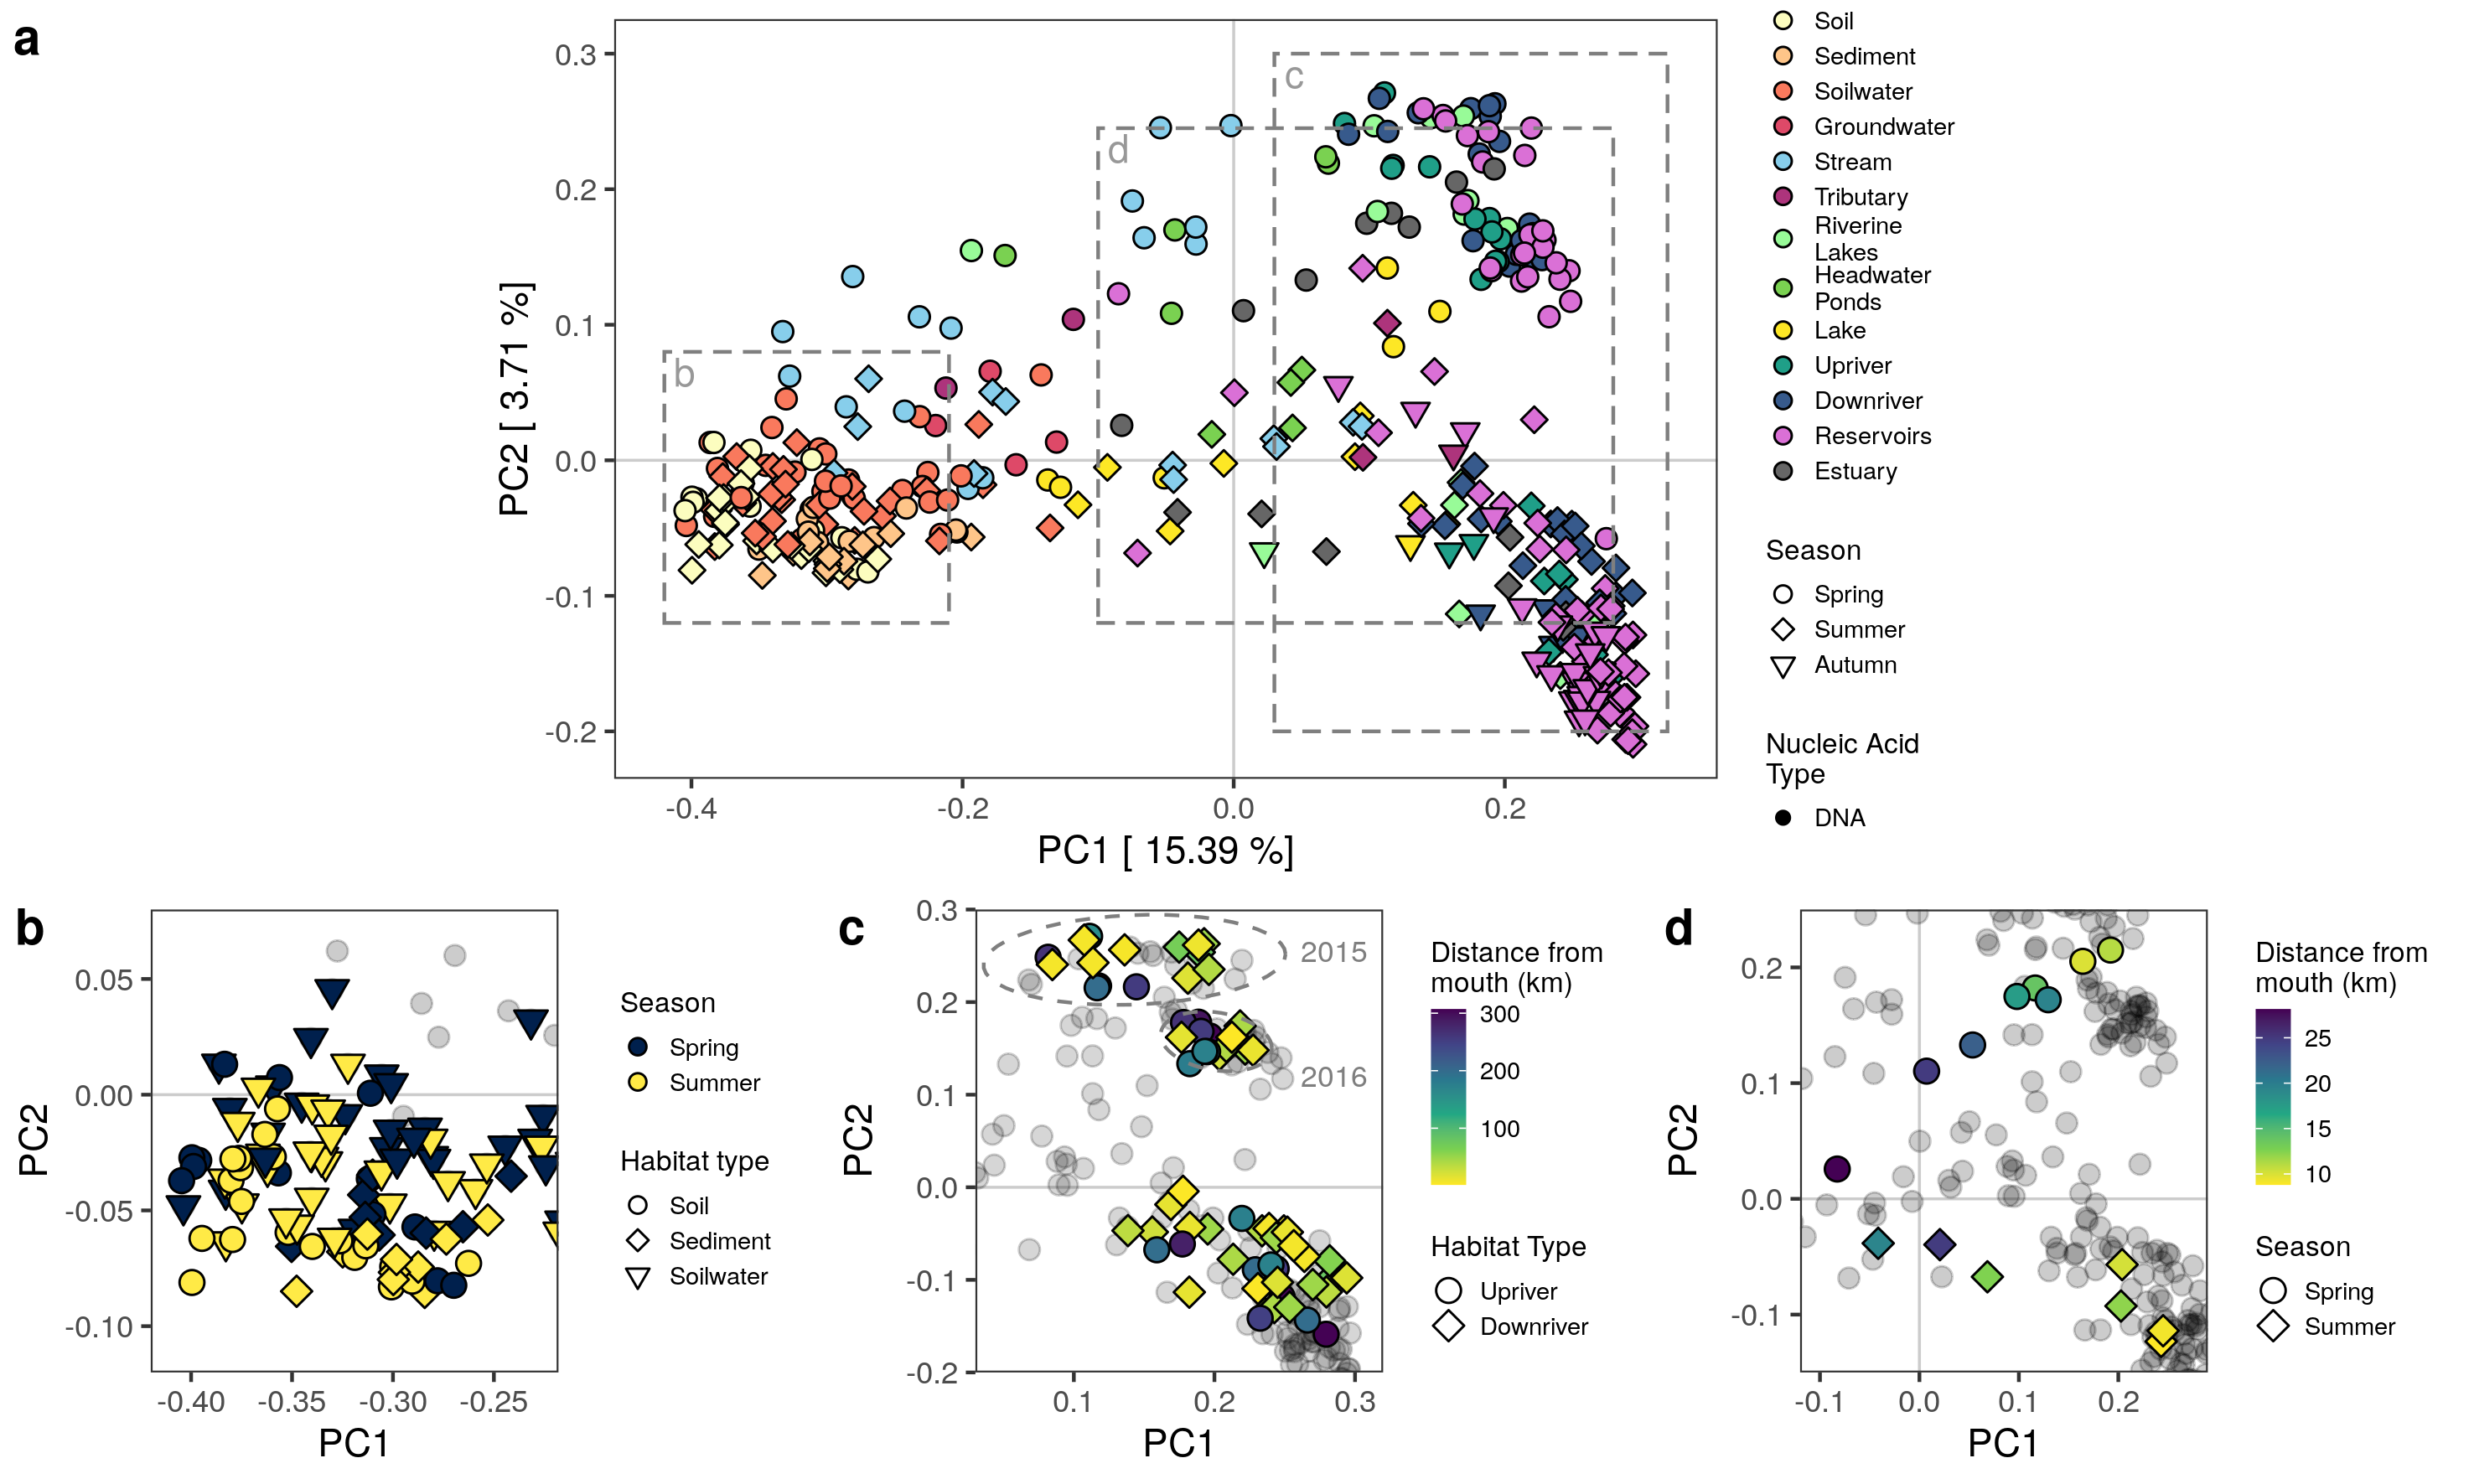
\includegraphics[width=16cm]{../../Figures/Final/PCoA_hellin_DNA_collage.png}
\caption{\textbf{Microbial community composition gradually changes along a terrestrial-hyrodlogical continuum and diverges between seasons.} Overall PCoA analysis of DNA samples (a) has been further explored with focus plots on terrestrial, riverine and estuary samples in panels b, c, d, respectively. Overall, the PCoA reveals microbial community shifts from terrestrial to freshwater samples. Spring and summer-autumn show distinct paths in multivariate space. Percentage of variance explained are given in square brackets for the first and second axes.}
%includegraphics[width=1\textwidth]
\end{figure}

\begin{figure}[!ht]
\centering
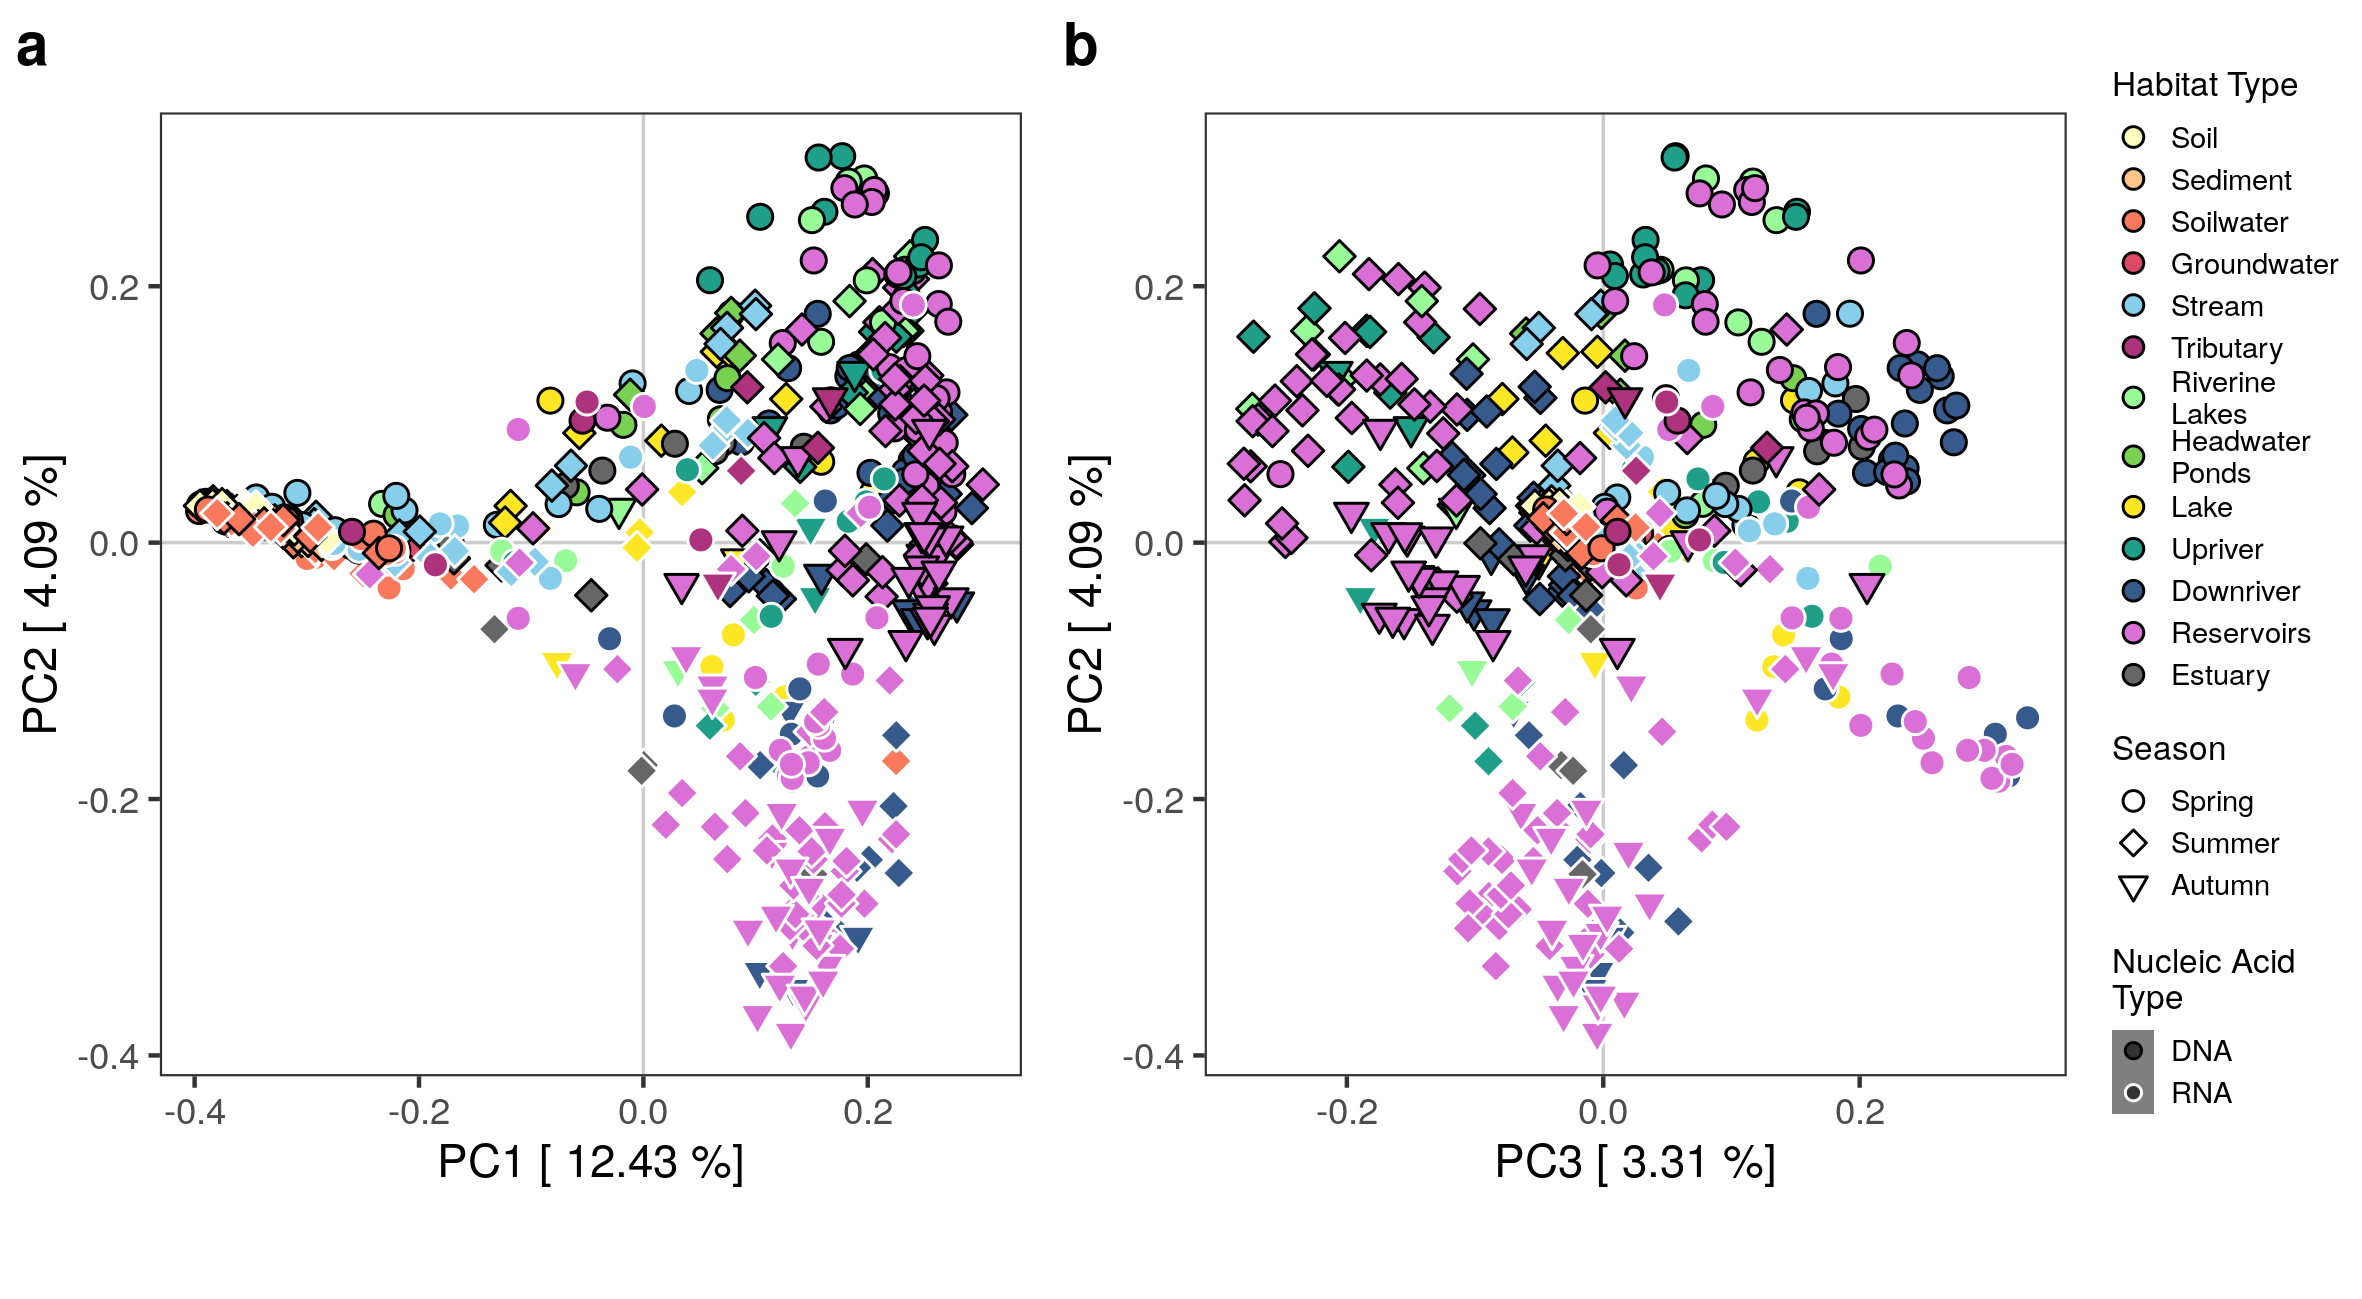
\includegraphics[width=17cm]{../../Figures/Final/PCoA_all_SampleType.png}
\caption{\textbf{RNA assemblages diverge from DNA within aquatic habitats, less so in terrestrially influenced habitats.} PCoA analysis including RNA samples. a) Visualisation of first and second axis of PCoA, differentiating habitat type and nucleic acid type, respectively. b) Different view on PCoA analysis using the second and third axis, differentiating nucleic acid type and seasons, respectively. Percentage of variance explained by the corresponding axes are given in square brackets.}
%includegraphics[width=1\textwidth]
\end{figure}

\begin{figure}[!ht]
\centering
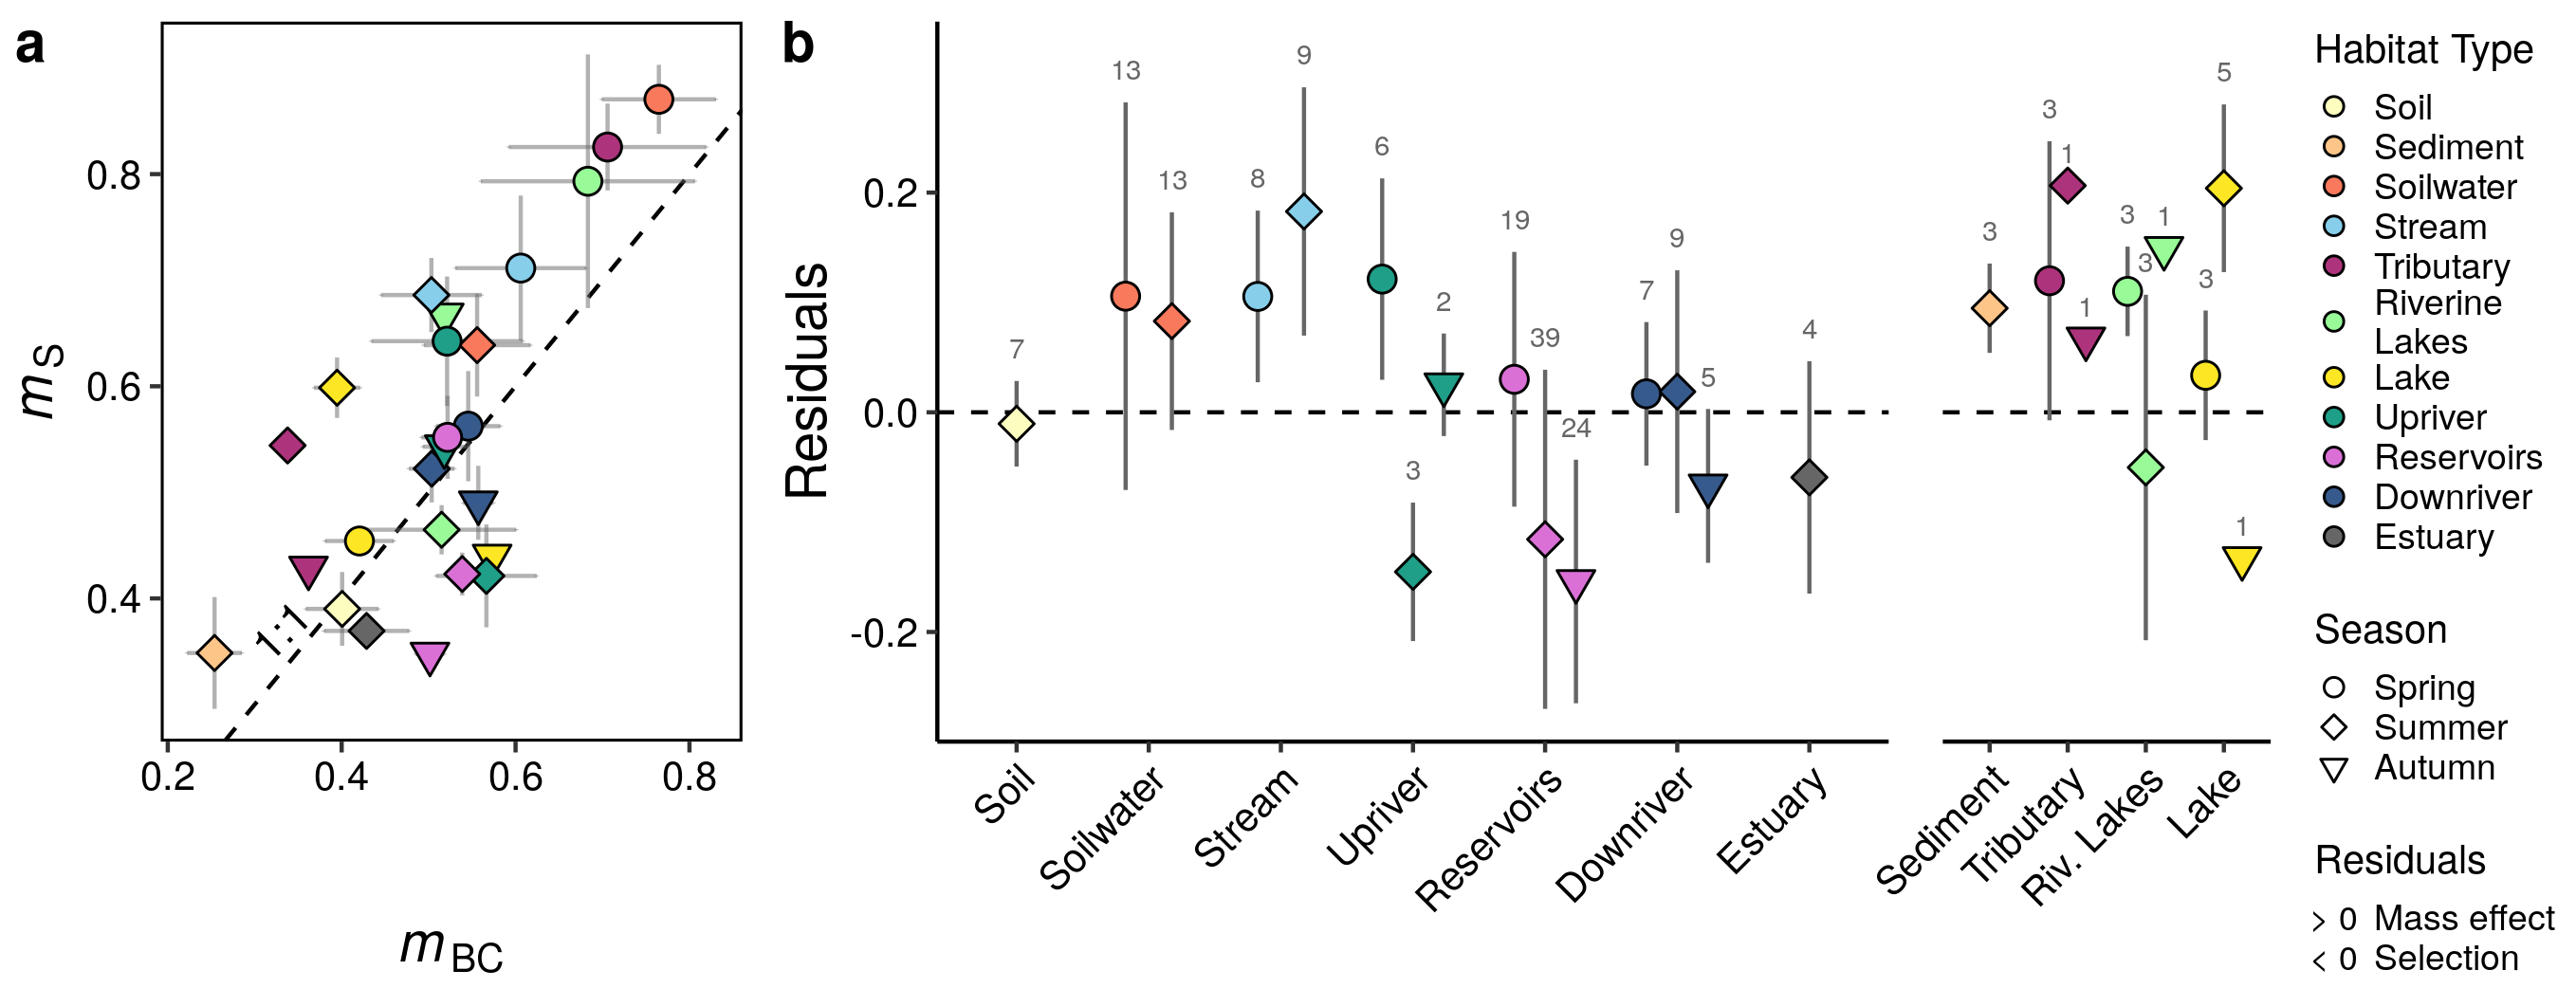
\includegraphics[width=15cm]{../../Figures/Final/distBCS_residcontinuum.png}
\caption{\textbf{Residuals to m\textsubscript{S} and m\textsubscript{BC} 1:1 line reveal transition from mass effects to species sorting along the continuum.} a) Distance between DNA and RNA of the same sample based on S{\o}rensen dissimilarity (\textit{m}\textsubscript{S}) against distance calculated with Bray-Curtis dissimilarity (\textit{m}\textsubscript{BC}). Distance was calculated within the axes capturing 75 \% of the variance in both PCoAs using different dissimilarity measures. b) Residuals to 1:1 line between m\textsubscript{S} and m\textsubscript{BC} along the terrestrial-aquatic continuum. Habitats outside of the direct continuum are given separately. Points represent the arithmetic mean and error bars represent the standard error (a) and standard deviations from the mean (b). Sample sizes of each point are indicated above the points. Sample sizes are equivalent in panels a and b.}
%includegraphics[width=1\textwidth]
\end{figure}

\begin{figure}[!ht]
\centering
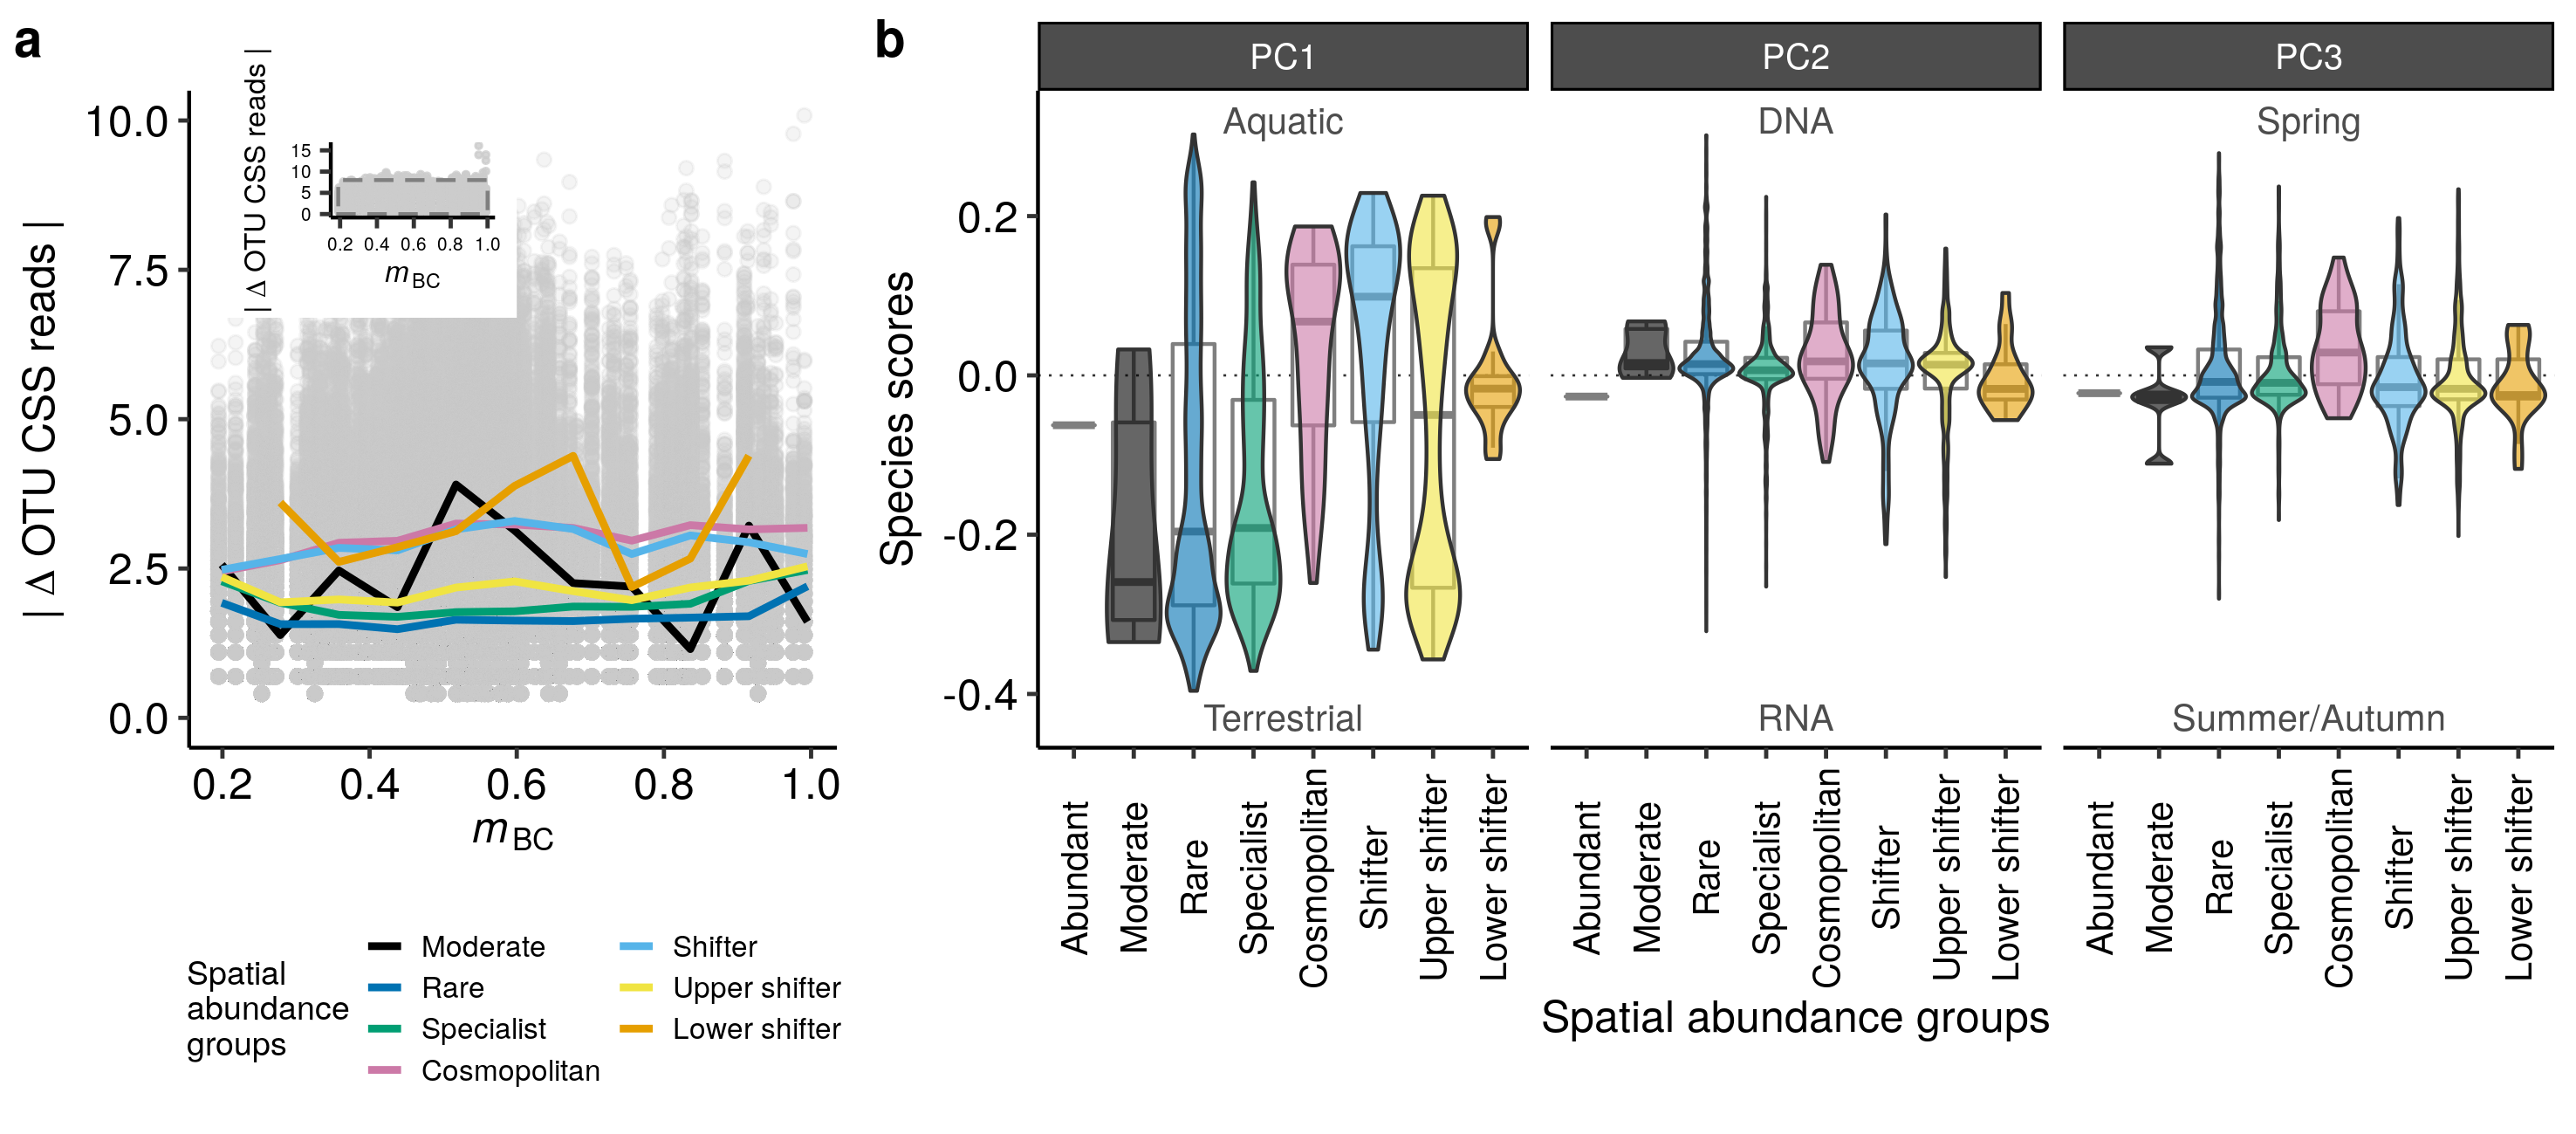
\includegraphics[width=15cm]{../../Figures/Final/abgroups_rollmean_violin}
\caption{\textbf{DNA and RNA dissimilarities arise through abundance differences across the rank abundance curve.} a) Difference in DNA and RNA abundance (CSS reads) against \textit{m}\textsubscript{BC}. Given are absolute values. Lines represent rolling means with bin size = 10. b) Boxplots and violin plots showing the distribution of species scores and thus OTU optima within PCoA space. The middle line represents the median, lower and upper hinges of boxplots correspond to the 25th and 75th percentiles. Upper and lower whiskers expand to the largest and smallest value, respectively, but no further than 1.5 times the inter-quartile range from the hinge. There were a plethora of outliers that lie beyond the whiskers for all boxes and thus, were removed for visualisation purposes. Violin plots visualise the probability density distribution smoothed by a kernel density estimator.}
%includegraphics[width=1\textwidth]
\end{figure}


\end{document}
